\chapter{Implementacija i korisničko sučelje}
		
		
		\section{Korištene tehnologije i alati}
		
		
			Komunikacija unutar tima odvijala se putem aplikacija \underline{WhatsApp}\footnote {\url{https://www.whatsapp.com/}} i \underline{Discord} \footnote{\url{https://discord.com}}, a s profesorom smo komunicirali putem \underline{MS Teamsa} \footnote{\url{https://www.microsoft.com/hr-hr/microsoft-teams/group-chat-software/}}.
			
			
			Za izradu UML dijagrama korišten je alat \underline{Astah Professional} \footnote {\url{https://astah.net/downloads/}} (studentska licenca), a za izradu ER dijagrama javno dostupan alat \underline{dbdiagram} \footnote {\url{https://dbdiagram.io/home}}.
			
			Verzioniranje koda olakšale su nam platforme \underline{Git} \footnote {\url{https://git-scm.com/}}  i \underline{GitLab} \footnote {\url{https://gitlab.com/}}  na kojem je dostupan udaljeni repozitorij s kojeg i na koji članovi razvojnog tima mogu preuzimati/postavljati kod i projektnu dokumentaciju.
			
			 Dokumentacija je pisana unutar okoline \underline{TeXstudio} \footnote {\url{https://www.latex-project.org/}} koja olakšava pisanje u \underline{LaTeX-u} \footnote {\url{https://www.texstudio.org/}} koji omogućuje izradu strukturiranog i preglednog dokumenta.
			
		
			Članovi tima su koristili razvojno okruženje s kojim su od ranije upoznati, \underline{Microsoft Visual Studio } \footnote {\url{https://visualstudio.microsoft.com/}}. Integrirana razvojna okruženja (\textit{engl. integrated development environment (IDE)}) programerima pružaju grafičko sučelje za pisanje koda u različitim programskih jezicima, usporedni pregled različitih projekata i druge pogodnosti poput uočljivog formatiranja koda i olakšanog otkrivanja i ispravljanja pogrešaka. 
			
			Osim ručnog testiranja aplikaciju smo testirali pomoću radnog okvira \underline{Selenium} \footnote {\url{https://www.selenium.dev/}}. Važno je biti svjestan da je nepostojanje pogreške, bez formalne verifikacije, nemoguće utvrditi.
			
			Poslužiteljska strana aplikacije implementirana je koristeći radni okvir za razvoj web aplikacija \underline{Django } \footnote {\url{https://www.djangoproject.com/}}(jezik \underline{Python 3.8} \footnote {\url{https://www.python.org/downloads/}}). Prednosti uporabe ovog (i sličnih) radnih okvira su olakšana implementacija čestih funkcionalnosti, komunikacija s bazom podataka, osigurana određena razina sigurnosti i općenito olakšana izgradnja programske potpore. Za bazu podataka odabrana je baza \underline{PostgreSQL }\footnote {\url{https://www.postgresql.org/}},  na glasu kao pouzdana i robusna relacijska baza podataka.
			Za izradu klijentske strane tradicionalno je korišten \underline{HTML}\footnote {\url{https://developer.mozilla.org/en-US/docs/Web/HTML}}, \underline{CSS}\footnote {\url{https://www.w3.org/Style/CSS/Overview.en.html}} i \underline{JavaScript} \footnote {\url{	https://www.javascript.com/}}. Izradu korisničnog sučelja olakšao nam je razvojni okvir \underline{Bootstrap}\footnote {\url{https://getbootstrap.com/}} s mnoštvom javno dostupnih stilova za često korištene HTML elemente. Pri dizajniranju izgleda stranice korištene su i SVG ikonice javno dostupne na stranici \underline{FreeSVG} \footnote {\url{https://freesvg.org/}}. 
		
			Radi pouzdanosti i neovisnosti aplikacije obavljena je virtualizacija korištenjem platforme\underline{ Docker} \footnote {\url{https://www.docker.com/}}, a objavljena je na javnom poslužitelju pomoću \underline{Digital Oceana} \footnote {\url{https://www.digitalocean.com/}}, brzorastuće platforme zasnovane na računarstvu u oblaku (\textit{engl. cloud computing}), koja između ostalih pruža uslugu objave aplikacija (\textit{engl. cloud hosting}). Na poslužitelju, tzv. \textit {dropletu}, konfigurirali smo dva kontejnera, jedan za aplikaciju i jedan za bazu podataka. \newline

		
			
			Temeljna je svrha svih navedenih tehnologija i alata ubrzati i pojednostaviti razvoj programske potpore visoke kvalitete.
					
			\eject 
		
	
		\section{Ispitivanje programskog rješenja}
			
		\subsection{Ispitivanje sustava}
			
			Za testiranje sustava odabran je radni okvir Selenium IDE\footnote{\url{https://www.selenium.dev/selenium-ide/}} radi njegove jednostavnosti korištenja te sličnosti ponašanju stvarnog korisnika. Odabrani testovi usredotočeni su na administrativne zadatke sustava i pokrivaju velik broj obrazaca uporabe.\\ 
			
			\noindent  \textbf{Ispitni slučaj 1: Dodavanje administratora}\\
			 \textbf{Ulaz:}
			 \begin{packed_enum}
			 	\item {Prijava u sustav kao administrator}
			 	\item {Ulaz u administracijsko sučelje klikom na gumb u izbornoj traci}
			 	\item {Unos neispravnih korisničkih podataka novog administratora}
			 	\item {Unos ispravnih korisničkih podataka novog administratora}
			 \end{packed_enum}
			 
			 
			 \textbf{Očekivani rezultat:}
			 \begin{packed_enum}
			 	\item {Uspješna prijava u sustav}
			 	\item {Otvaranje administracijskog sučelja}
			 	\item {Dojava greške o neispravnoj adresi e-pošte}
			 	\item {Potvrda o dostavi korisničkih podataka novog administratora na adresu e-pošte}
			 \end{packed_enum}
			 \textbf{Rezultat: }Prijava u postojeći administratorski račun je uspješna, unos neispravne adrese e-pošte pri unosu podataka novog administratora ispravno dojavljuje grešku, a prilikom unosa ispravnih korisničkih podataka ispravno se prikazuje potvrda o dostavljenim podatcima na adresu e-pošte. {\color{green} Aplikacija prolazi test.}
			 
			  \begin{figure}[H]
			 	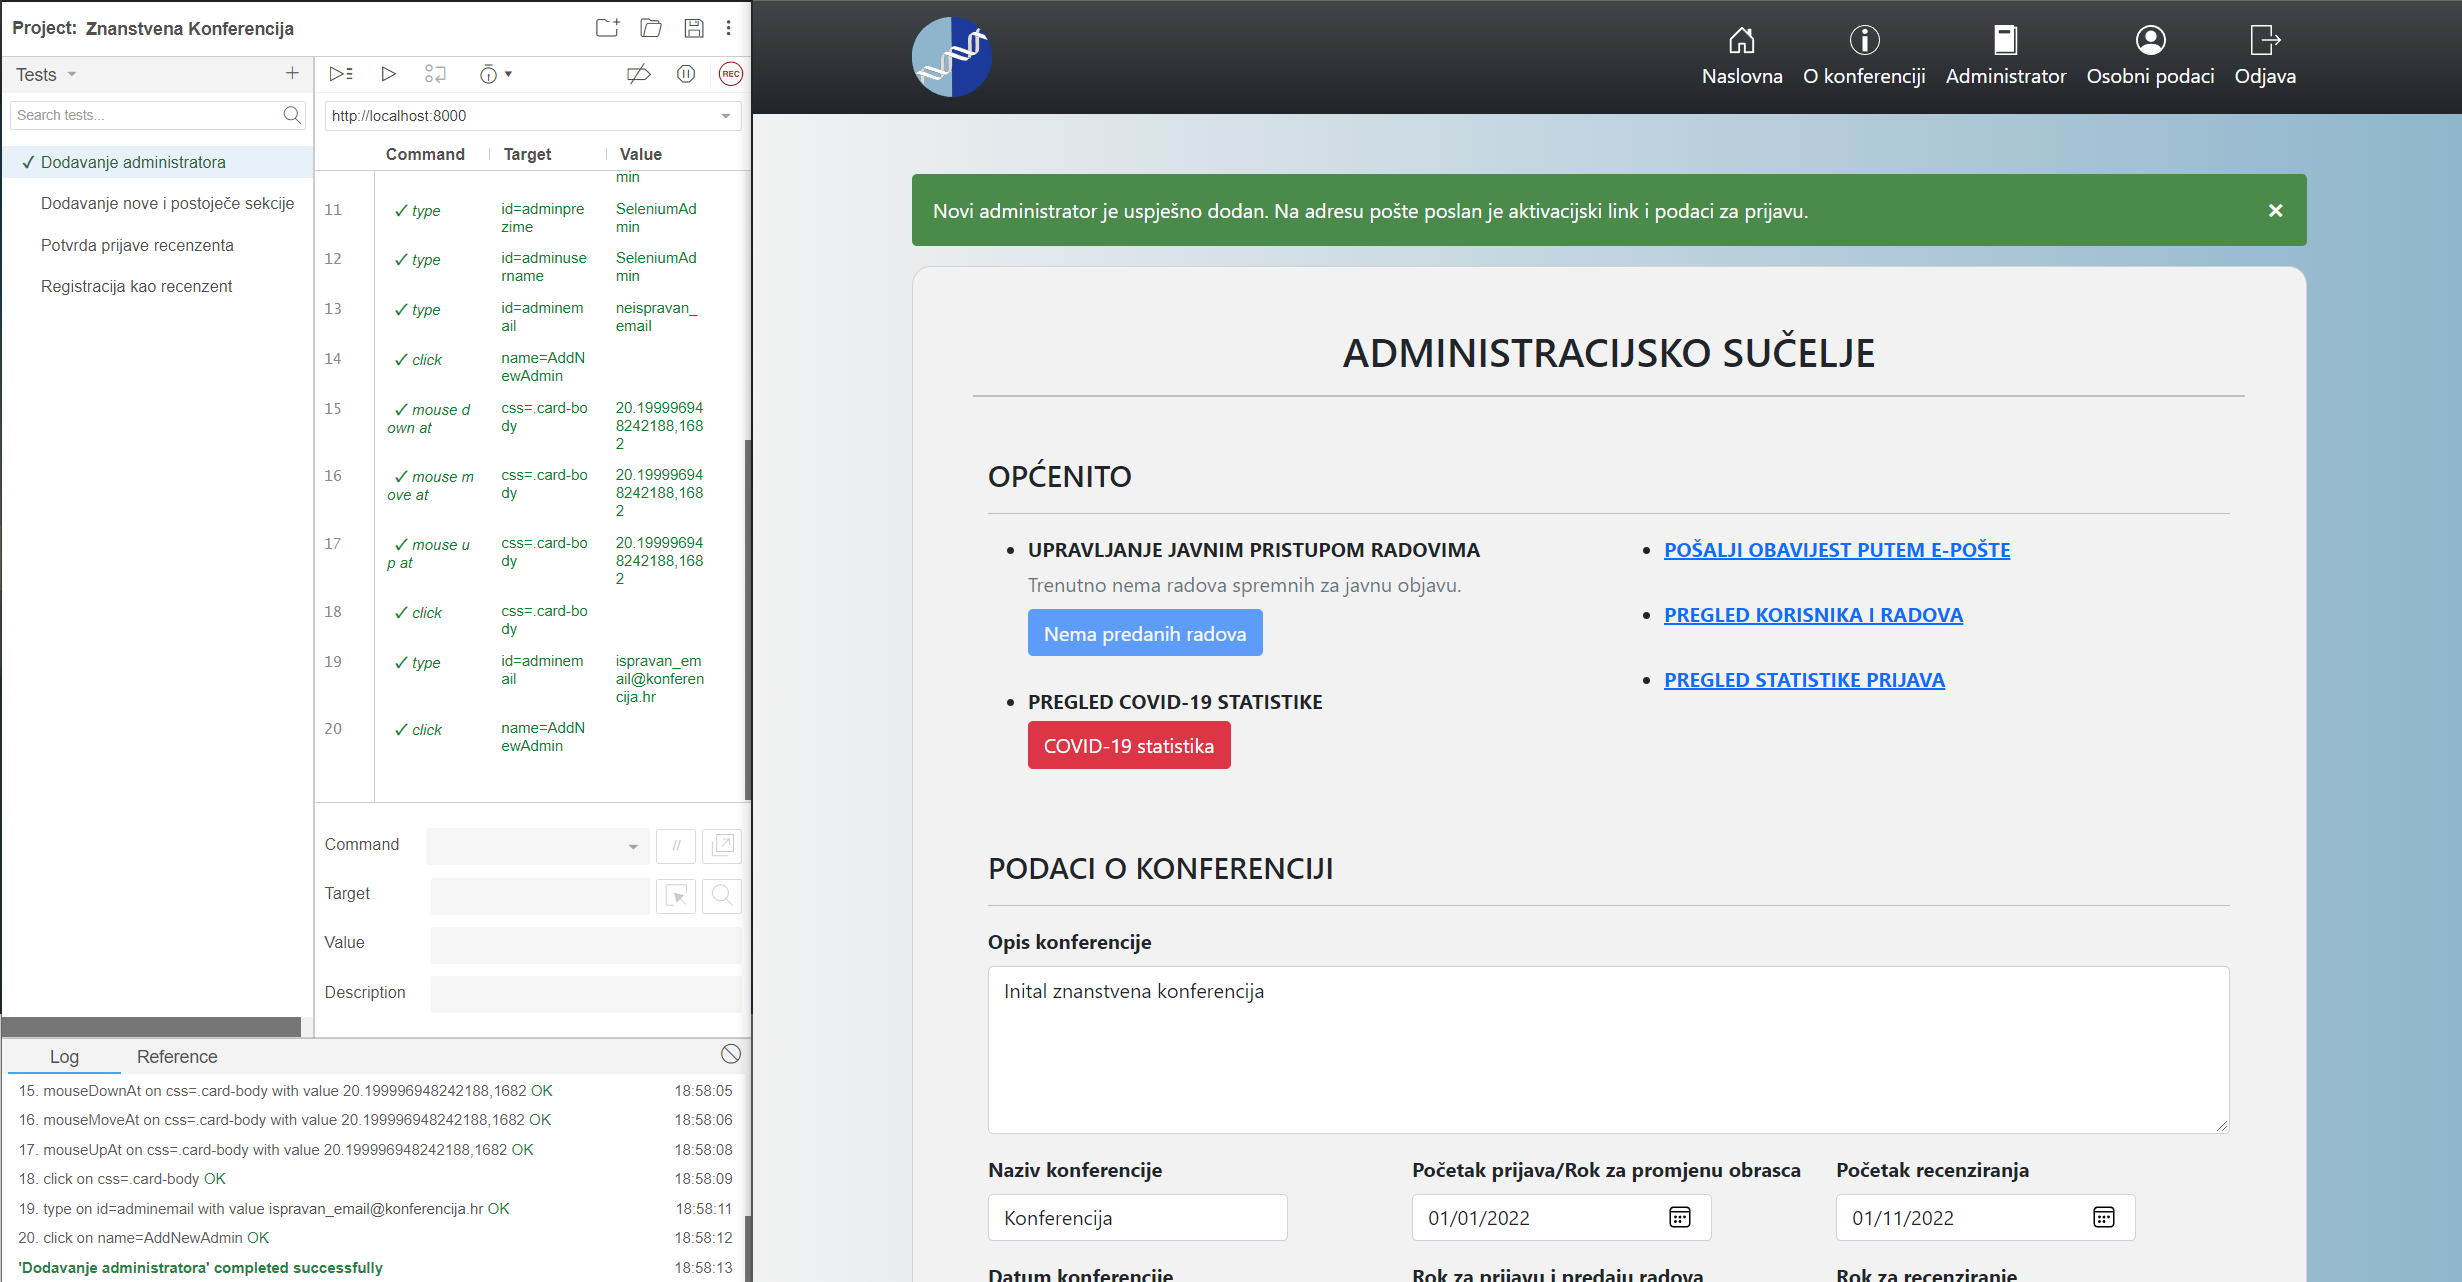
\includegraphics[width= 15 cm, height= 25 cm, keepaspectratio]{slike/test_dodavanje_administratora.png} 
			 	\centering
			 	\caption{Ispitni slučaj 1 - Dodavanje administratora}
			 	\label{fig:act5}
			 \end{figure}
			
			 \noindent \textbf{Ispitni slučaj 2: Dodavanje novih sekcija}\\
			 \textbf{Ulaz:}

			 \begin{packed_enum}
			 	\item {Prijava u sustav kao administrator}
			 	\item {Ulaz u administracijsko sučelje klikom na gumb u izbornoj traci}
			 	\item {Unos već postojeće sekcije}
			 	\item {Unos nove sekcije}
			 \end{packed_enum}

			 \textbf{Očekivani rezultat:}

			 \begin{packed_enum}
			 	\item {Uspješna prijava u sustav}
			 	\item {Otvaranje administracijskog sučelja}
			 	\item {Dojava greške o već postojećoj sekciji}
			 	\item {Nova sekcija dodanu u listu sekcija}
			 \end{packed_enum}

			 \textbf{Rezultat: }Prijava u postojeći administratorski račun je uspješna i otvara se administracijsko sučelje. Pokušaj dodavanja sekcije koja već postoji ispravno javlja pogrešku o pokušaju unosa već postojeće sekcije. Unos nove sekcije je uspješan i ispravno se dodaje na listu sekcija. {\color{green} Aplikacija prolazi test.}
			 
			   \begin{figure}[H]
			 	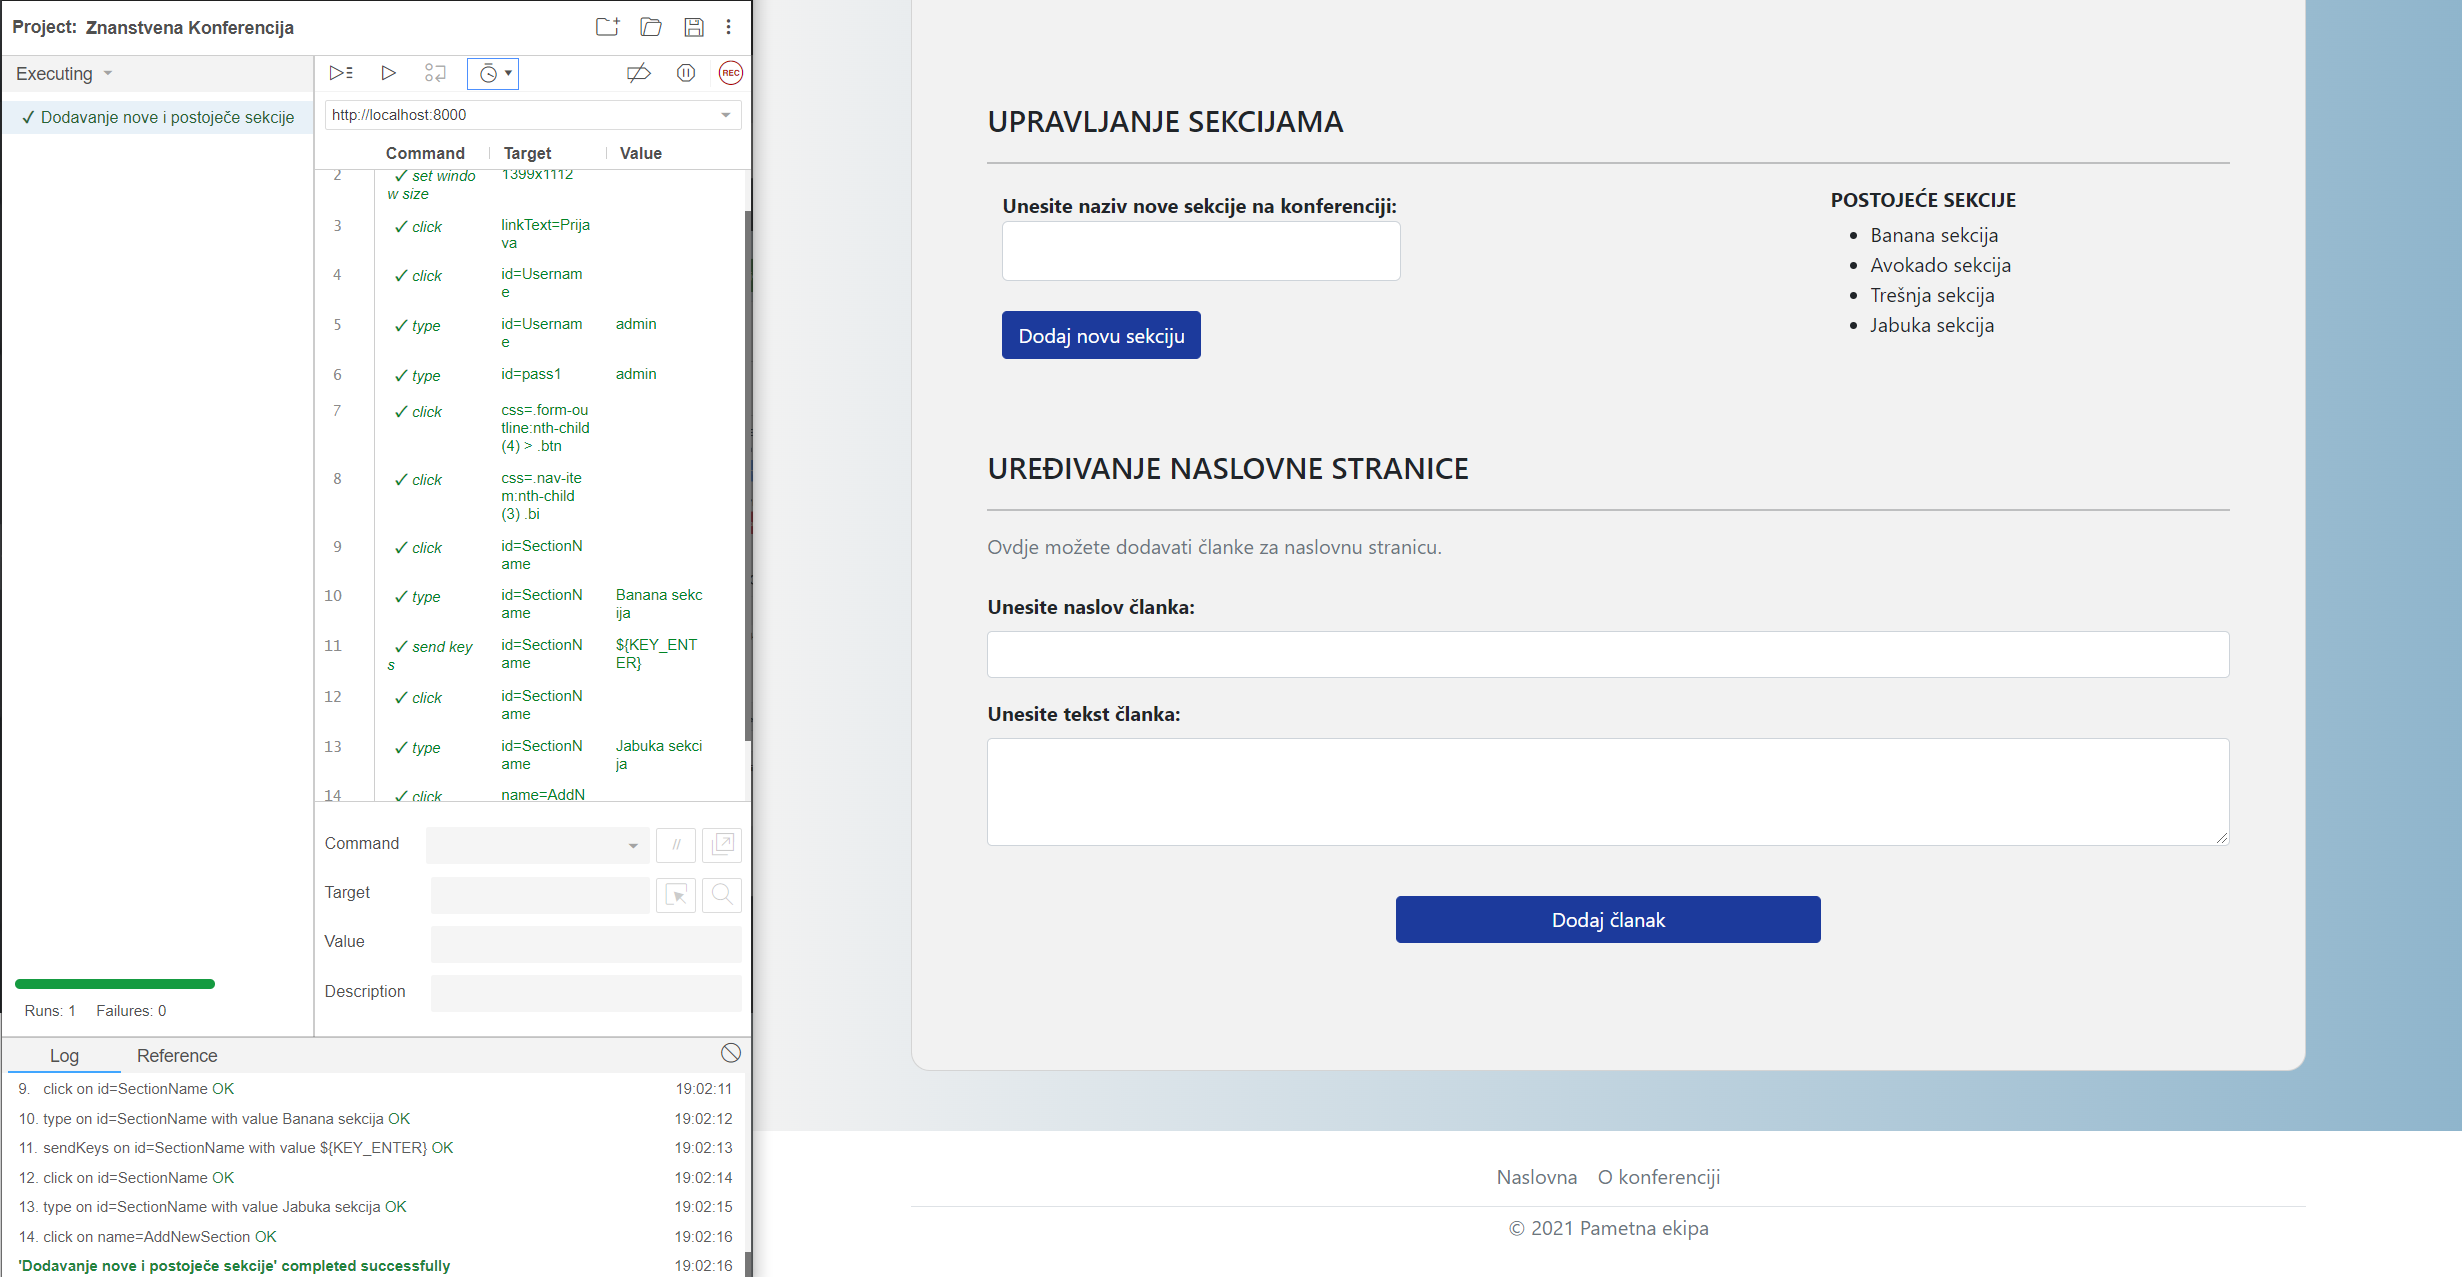
\includegraphics[width= 15 cm, height= 25 cm, keepaspectratio]{slike/test_dodavanje_sekcija.png} 
			 	\centering
			 	\caption{Ispitni slučaj 2 - Dodavanje novih sekcija}
			 	\label{fig:act5}
			 \end{figure}
			
			
			 \noindent \textbf{Ispitni slučaj 3: Registracija kao recenzent}\\
			  \textbf{Ulaz:}

			 \begin{packed_enum}
			 	\item {Klik na gumb za registraciju u izbornoj traci}
			 	\item {Unos podataka za registraciju}
			 	\item {Odabir registracije kao recenzent}
			 \end{packed_enum}

			 \textbf{Očekivani rezultat:}

			 \begin{packed_enum}
			 	\item {Otvara se sučelje za registraciju}
			 	\item {Odabirom registracije kao recenzent mijenjaju se polja obrasca prijave}
			 	\item {Obavijest o potrebi da predsjedavajući potvrdi registraciju}
			 \end{packed_enum}

			  \textbf{Rezultat: }Sučelje za registraciju otvara se nakon klika na gumb registracije. Nakon sto se označi gumb da se korisnik prijavljuje kao recenzent, obrazac prijave se mijenja i traži se odabir sekcije za koju se korisnik registrira. Po završetku prijave ispravno se javlja obavijest kako je potrebno da predsjedavajući potvrdi registraciju prije mogućnosti recenziranja. {\color{green} Aplikacija prolazi test.}
			  
			    \begin{figure}[H]
			 	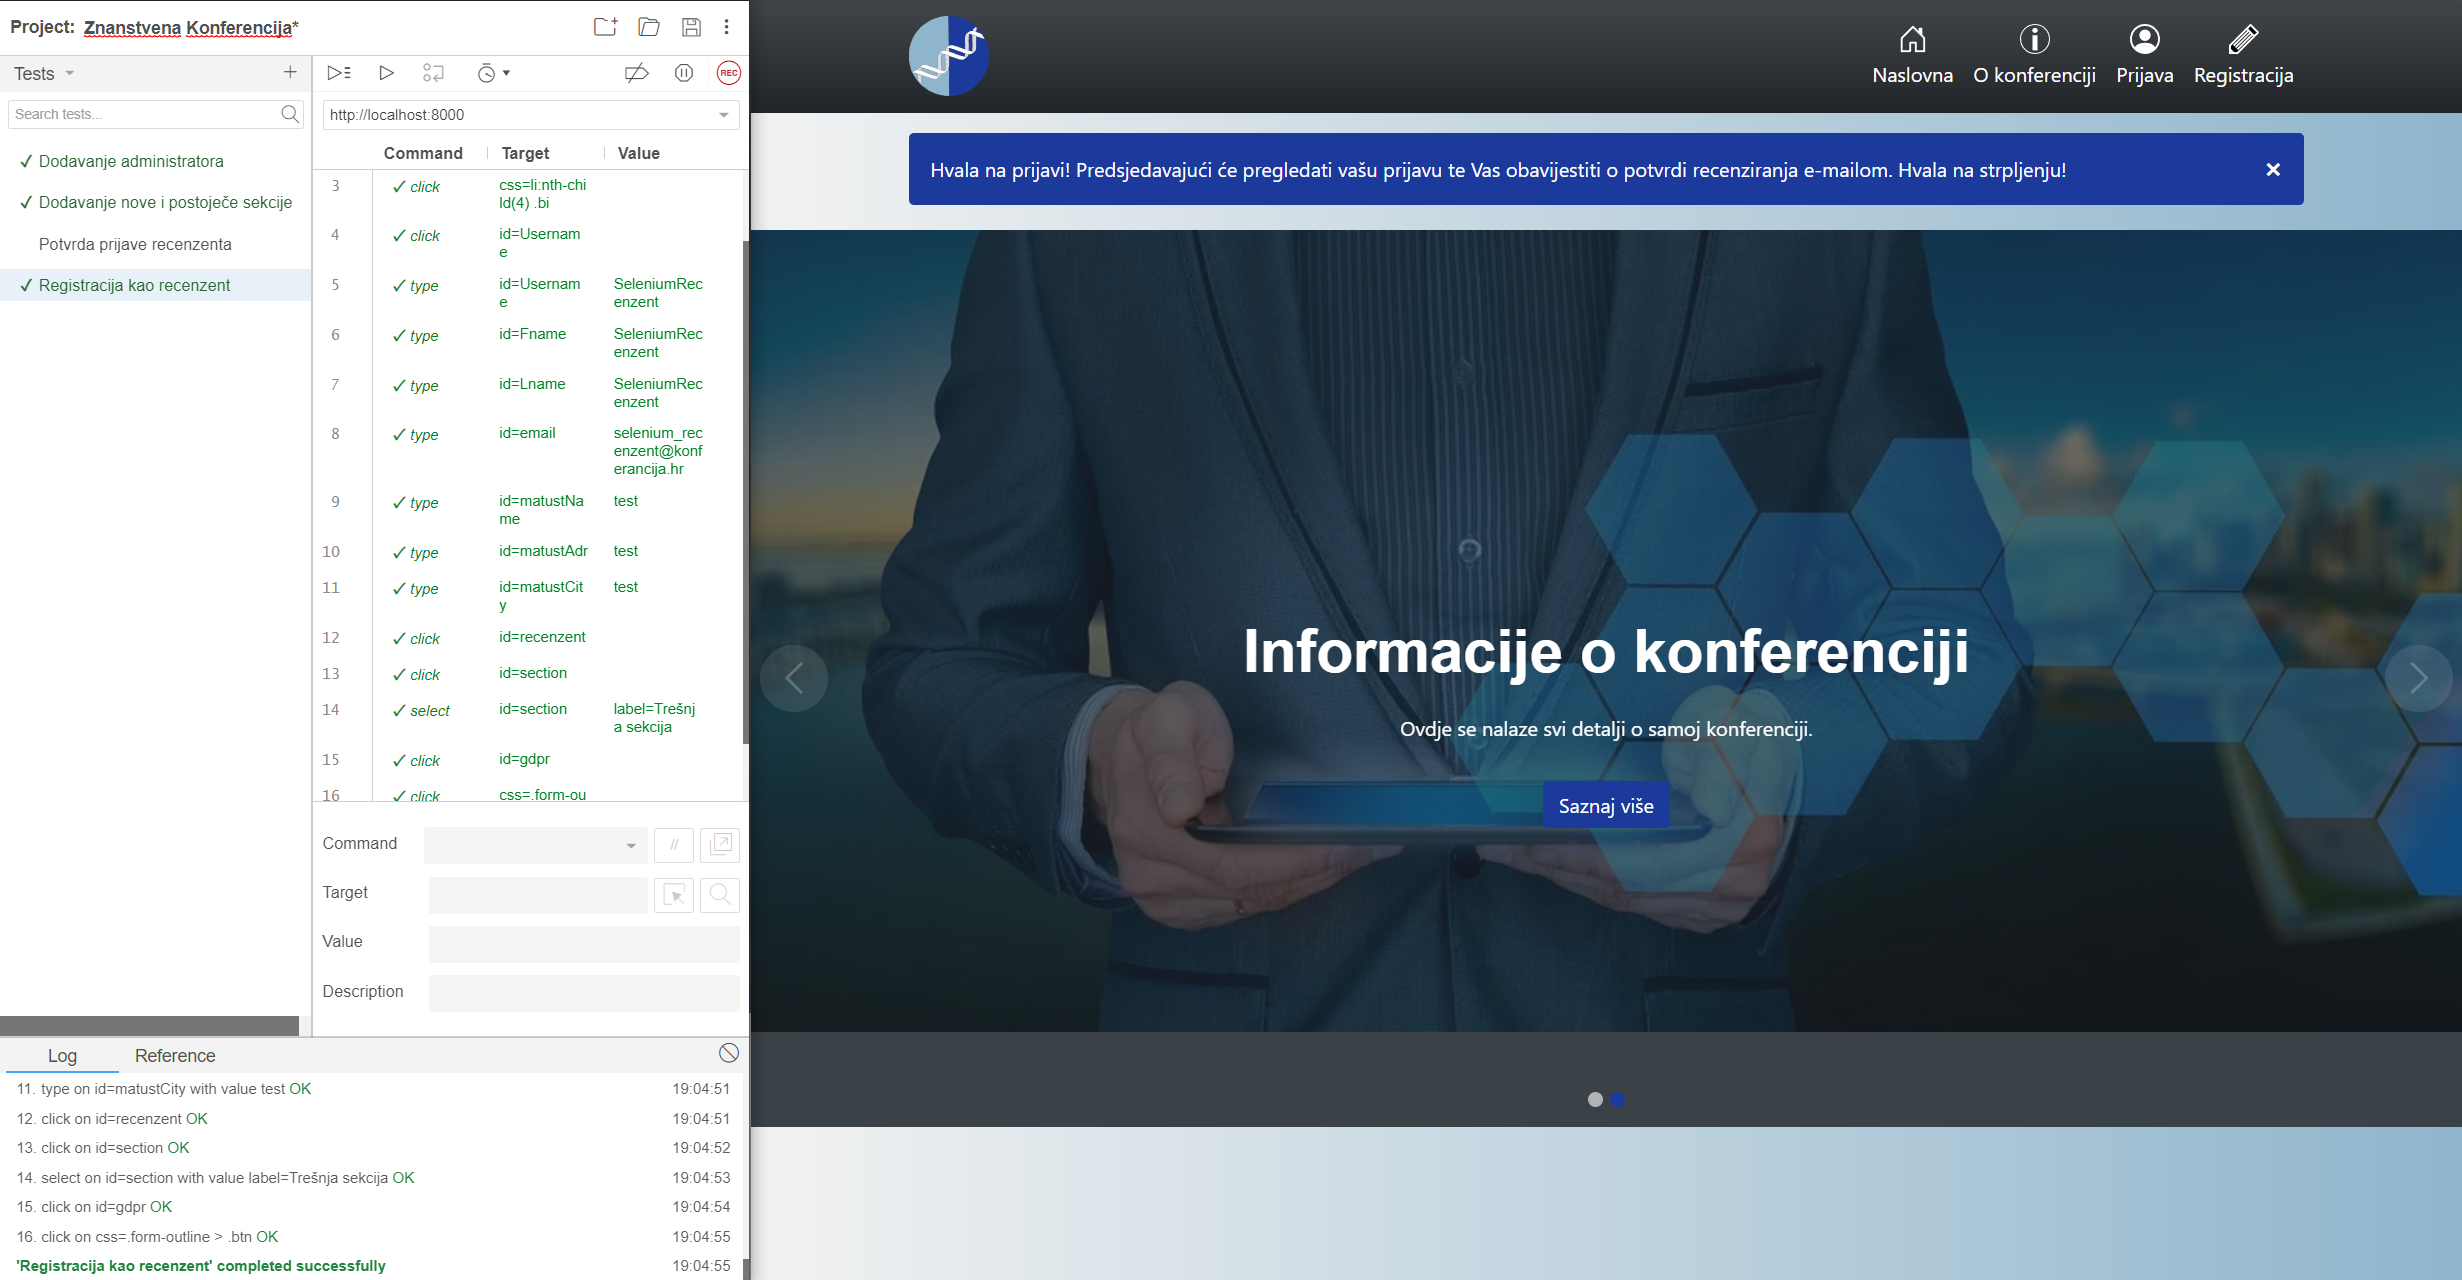
\includegraphics[width= 15 cm, height= 25 cm, keepaspectratio]{slike/test_registracija_kao_recenzent.png} 
			 	\centering
			 	\caption{Ispitni slučaj 3 - Registracija kao recenzent}
			 	\label{fig:act5}
			 \end{figure}
			
			
			 \noindent \textbf{Ispitni slučaj 4: Potvrda prijave recenzenta od strane predsjedavajućeg}\\

			  \textbf{Ulaz:}

			 \begin{packed_enum}
			 	\item {Prijava u sustav kao predsjedavajući}
			 	\item {Otvaranje upravljačkog sučelja}
			 	\item {Klik na gumb "Potvrdi"}
			 \end{packed_enum}

			  \textbf{Očekivani rezultat:}

			 \begin{packed_enum}
			 	\item {Izborna traka se mijenja i pojavljuje se gumb za otvaranje upravljačkog sučelja predsjedavajućeg}
			 	\item {Otvara se upravljačko sučelje predsjedavajućeg}
			 	\item {Prijava se prihvaća i recenzentu šalje se e-pošta s podacima za prijavu}
			 \end{packed_enum}

			 \textbf{Rezultat: }Prijavom kao predsjedavajući mijenja se izborna traka i pojavljuje se gumb za otvaranje upravljačkog sučelja predsjedavajućeg konferencije. Otvaranjem sučelja vidljiv je popis recenzenata koji čekaju potvrdu registracije. Klikom na gumb "Potvrdi" recenzentu se šalje e-pošta s potrebnim podacima za prijavu. {\color{green} Aplikacija prolazi test.}
			 
			   \begin{figure}[H]
			 	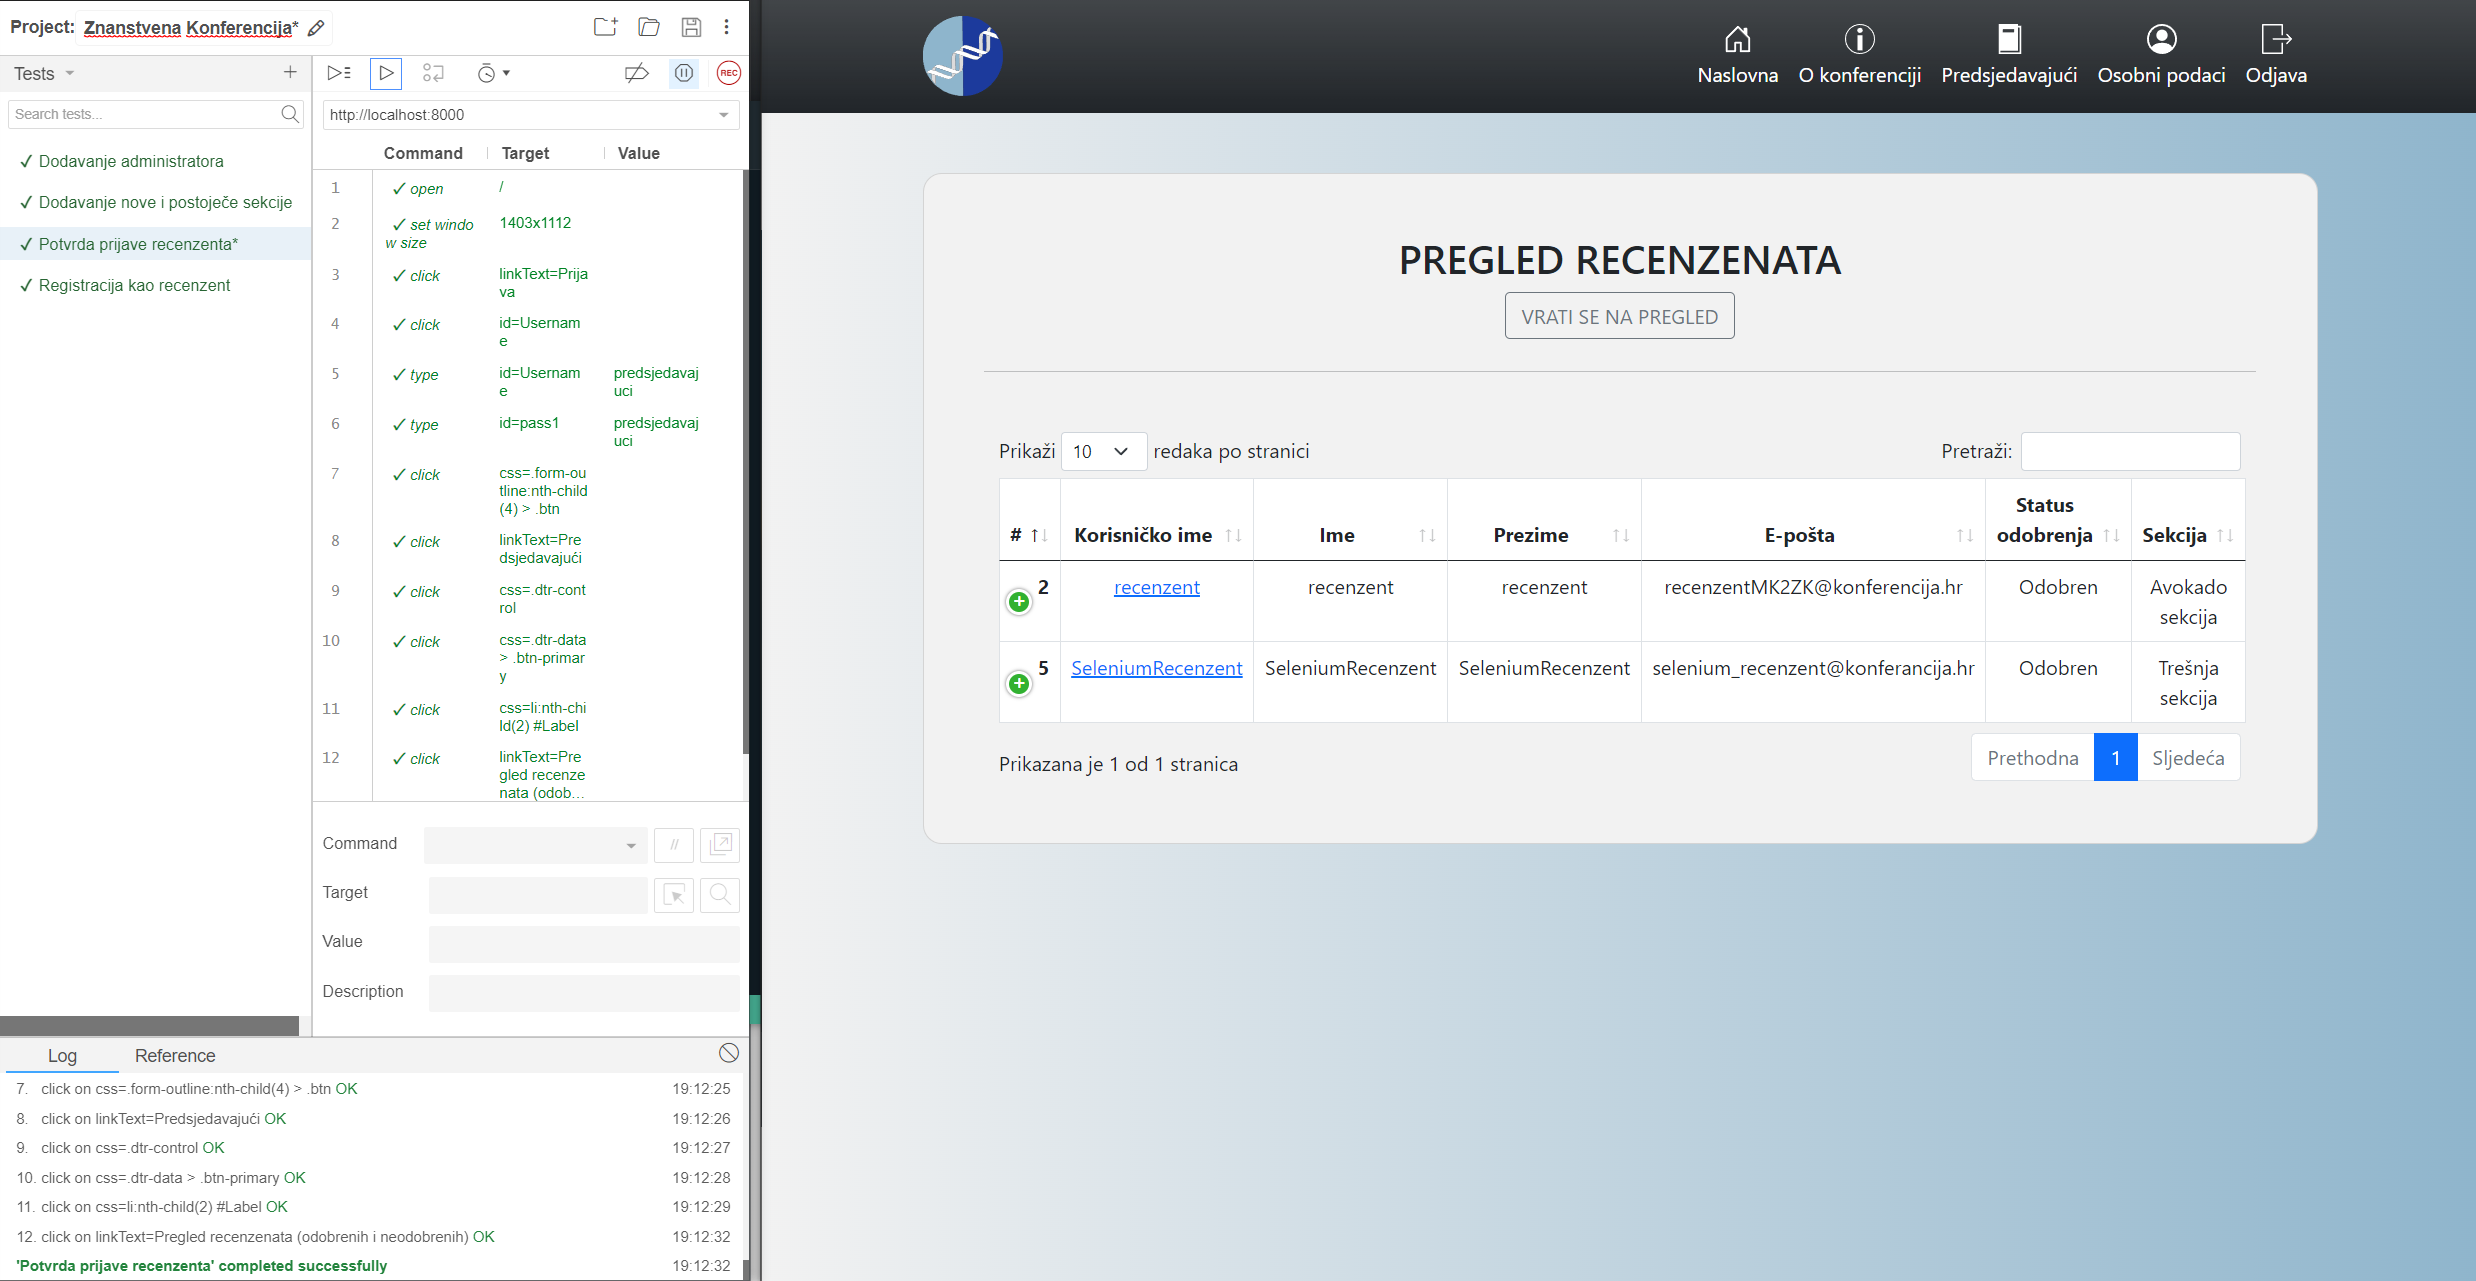
\includegraphics[width= 15 cm, height= 25 cm, keepaspectratio]{slike/test_potvrda_prijave_recenzenta.png} 
			 	\centering
			 	\caption{Ispitni slučaj 4 - Potvrda prijave recenzenta od predsjedavajućeg}
			 	\label{fig:act5}
			 \end{figure}
		
		

		
		\section{Dijagram razmještaja}
		
		Dijagram razmještaja opisuje fizičku organizaciju sustavu i programsku potporu koja se koristi na pojedinim dijelovima sustava. Klijent se sa svojeg računala spaja ne računalo poslužitelja uporabom proizvoljnog web preglednika, a sama komunikacija odvija se preko HTTP protokola. Računalo poslužitelja osim sa korisnikom komunicira i sa bazom podataka Svjetske zdravstvene organizacije od kuda dohvaća podatke o incidenciji Covid-19 virusa.
			 
			 
			\begin{figure}[H]
			 	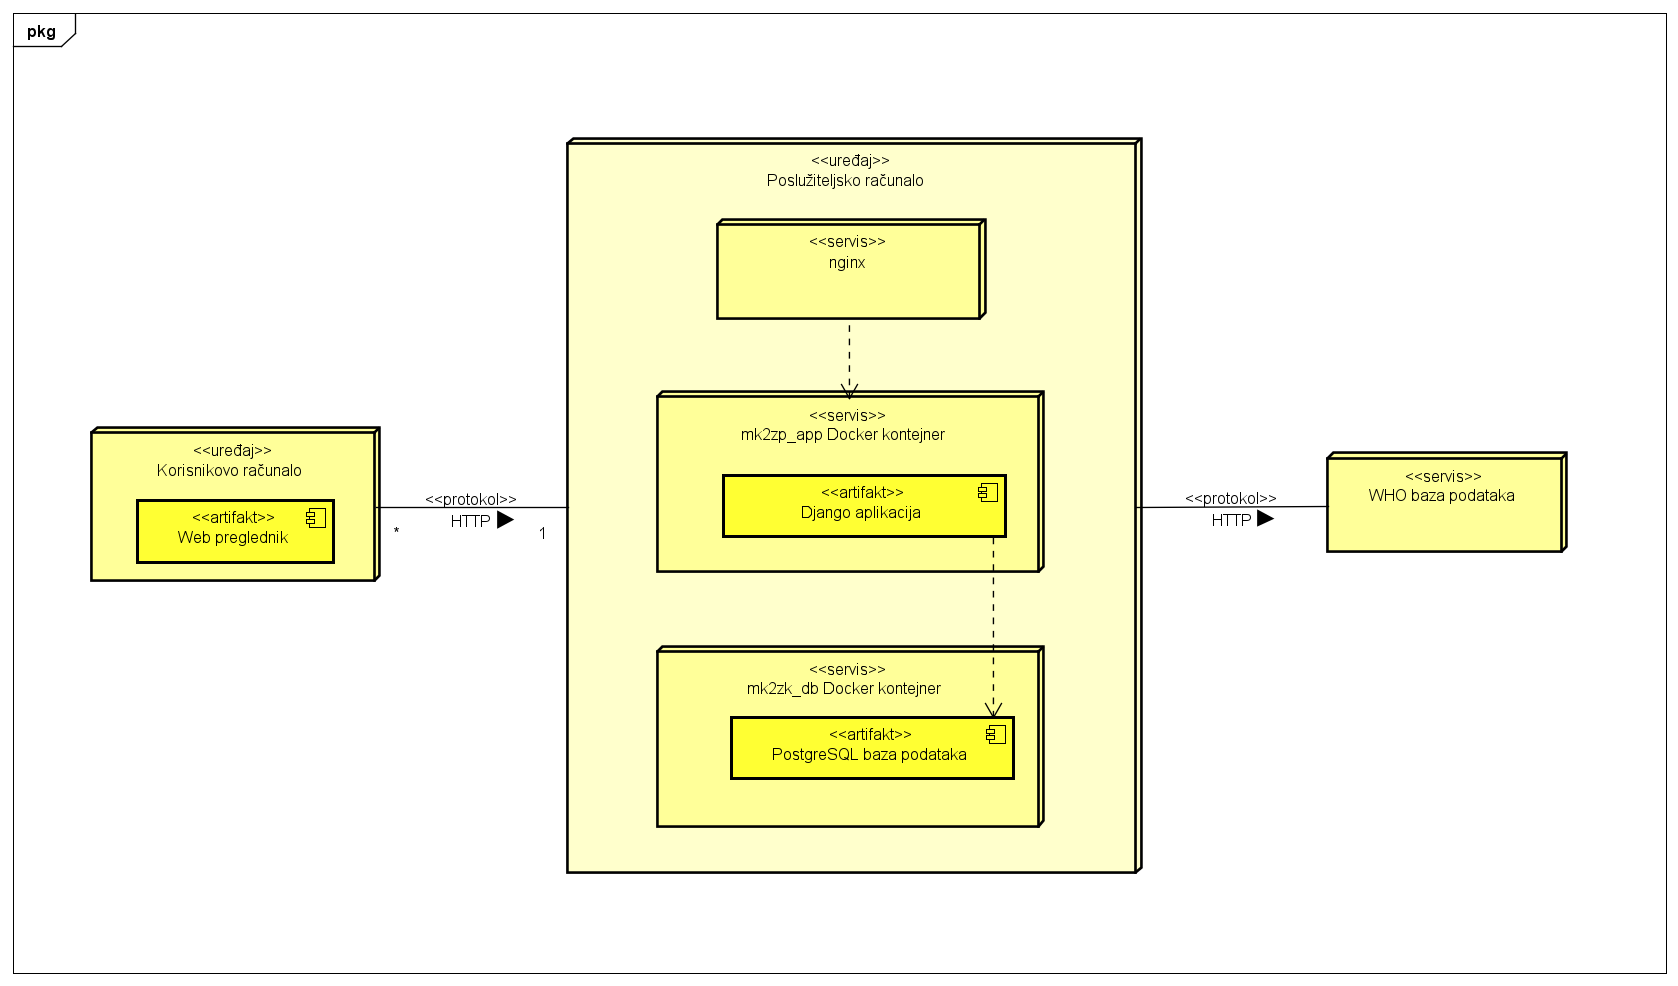
\includegraphics[width= 15 cm, height= 25 cm, keepaspectratio]{dijagrami/Diagram razmjestaja.png} 
			 	\centering
			 	\caption{Dijagram razmještaja - Znanstvena konferencija}
			 	\label{fig:act5}
			 \end{figure}

		
		\section{Upute za puštanje u pogon}

			\textbf{Instalacija alata Dockera i git-a}

			Potrebno je preuzeti alat Docker (za Windows i Mac sustave) i instalirati ga. Za Linux sustave isto je moguće napraviti pomoću naredbe \verb|sudo apt-get install docker-ce docker-ce-cli containerd.io| Također je potrebno preuzeti i instalirati Git.

			Potrebno je pozicionirati se u mapu u koju želimo klonirati repozitorij aplikacije naredbom \verb|git clone https://gitlab.com/fotoModeli/znanstvenakonferencija.git|. Nakon toga potrebno je preimenovati datoteku \textit{.env.example} u \textit{.env} datoteku te popuniti navedene varijable. Napokon, potrebno je pozicionirati se u mapu \textit{znanstvenakonferencija} i pokrenuti naredbu \verb|docker-compose up -d --build|.

			Također je vrlo bitno da u datoteci docker-entrypoint.sh, koja se nalazi u mapi \textit{IzvorniKod} način čitanja datoteke promijenimo iz CRLF u LF (Unix). Ukoliko je datoteka već postavljena na LF, isto nije potrebno mijenjati.

			\textbf{Instalacija Django-a}

			Za instalaciju alata Django prvo je potrebno preuzeti i instalirati Python. Pod pretpostavkom da je izvršen prethodni korak i time kloniran sadržaj aplikacije lokalno (naredbom \verb|git clone|), sljedeće što je potrebno je pozicionirati se u radni direktorij repozitorija i pokrenuti naredbu python -m venv venv. Nakon toga aktivacija virtualnog okruženja vrši se naredbom \verb|venv \textbackslash Scripts \textbackslash activate|.

			Nakon navedenog, potrebno je pozicionirati se u mapu \textit{IzvorniKod} i instalirati potrebne pakete naredbom \verb|pip install -r requirements.txt| te nakon toga, server je moguće lokalno (ili produkcijski) pokrenuti naredbom \verb|python manage.py runserver| 
		\eject
		
			\textbf{Konfiguracija web poslužitelja, baze podataka i poslužitelja baze podataka}\\

			Prethodni odsječci opisuju pokretanje servera s alatom Docker, koji znatno olakšava lokalno (i produkcijsko) pokretanje aplikacije. To je primjetljivo jer je za pokretanje servera potrebno samo klonirati git repozitorij te u komandnu liniju unijeti samo nekoliko naredbi.
			
			
			\eject 